% ==========================================================================
%  Chapter 69 — RC Beam Validation: Ko-Bathe Concrete 3D Sub-Model
% ==========================================================================

\chapter{Validation of the 3D Continuum Sub-Model with Imposed Rotation}
\label{ch:rc-beam-validation}

The reinforced-concrete sub-model pipeline developed in
Chapters~\ref{ch:ko-bathe-3d}--\ref{ch:reinforced-submodel} is designed
to resolve the nonlinear material behaviour inside each beam cross-section
of the global structural model.  During a multiscale analysis, the
\texttt{SubModelSolver} receives incremental boundary conditions derived
from the global beam kinematics---primarily curvatures and axial strains
that translate into imposed displacements on the faces of a prismatic
finite-element domain.

This chapter validates the complete sub-model infrastructure by solving a
standalone boundary-value problem: a doubly-clamped prismatic RC beam
loaded by an incremental rotation imposed on one of its end faces.  Two
cases are compared:

\begin{enumerate}
  \item[\textbf{Case A.}] \textbf{Plain concrete} (hex8 elements only),
        exercising the Ko--Bathe three-dimensional plastic-fracturing
        model in pure bending.
  \item[\textbf{Case B.}] \textbf{Reinforced concrete} (hex8 + embedded
        truss rebar), testing the \texttt{MultiElementPolicy} assembly
        and the tension-stiffening effect of embedded steel bars.
\end{enumerate}

The test reproduces---under controlled, quasi-static conditions---the
exact loading pattern that the sub-model solver encounters during the
global analysis: a linearly ramped displacement field on one face,
with the opposite face fully clamped.


% =========================================================================
\section{Geometry and Material Properties}
\label{sec:rcbeam-geometry}

The test specimen is a prismatic beam with dimensions
$0.30 \times 0.40 \times 2.00$~m (width $\times$ height $\times$ span).
The cross-section is discretised with a $4\times4$ grid, and 16~elements
along the span, giving a total of $4\times4\times16 = 256$ hex8 elements.

\paragraph{Concrete.}
The Ko--Bathe three-dimensional plastic-fracturing model with
$f'_c = 30$~MPa.  All parameters are derived internally from~$f'_c$
as described in Chapter~\ref{ch:ko-bathe-3d}.

\paragraph{Reinforcement (Case~B only).}
Eight longitudinal bars of $\diameter 20$~mm ($A_s = 3.14\times10^{-4}$~m$^2$
each) placed at the four corners and four mid-faces of the cross-section,
one element inset from the edge to approximate concrete cover.
Each bar is discretised into 16 truss segments---one per element along
the span---producing 128~line elements. The steel follows the
Menegotto--Pinto model with:
%
\[
  E_s = 200{,}000~\text{MPa}, \quad
  f_y = 420~\text{MPa}, \quad
  b   = 0.01, \quad
  R_0 = 20, \quad
  cR_1 = 18.5, \quad
  cR_2 = 0.15.
\]

The reinforced model contains $256 + 128 = 384$ elements assembled
in a heterogeneous \texttt{FEM\_Element} vector managed by
\texttt{MultiElementPolicy}.


% =========================================================================
\section{Boundary Conditions and Loading}
\label{sec:rcbeam-loading}

The loading scheme reproduces the boundary-condition pattern that the
sub-model solver applies when beam section kinematics change between
global analysis steps:

\begin{itemize}
  \item \textbf{MinZ face} (at $z = 0$): all three displacement components
        constrained to zero (clamped).
  \item \textbf{MaxZ face} (at $z = L$): a rotation $\theta_y$ about the
        local $Y$-axis is imposed through rigid-section kinematics:
        %
        \begin{equation}\label{eq:rcbeam-bc}
          u_x = 0, \qquad
          u_y = 0, \qquad
          u_z = -\theta_y \, (x - x_c),
        \end{equation}
        %
        where $x_c$ is the centroid of the MaxZ face.  The displacement
        pattern is consistent with the plane-sections-remain-plane
        assumption used in beam theory.
\end{itemize}

The rotation ramps linearly from $0$ to $\theta_{\max} = 5$~mrad
($\approx 0.29°$) over 40~equal increments.  The incremental solver
uses Newton--Raphson iteration (PETSc SNES with LU preconditioner)
with up to 8~levels of automatic bisection for non-convergent steps.

The \texttt{CustomControl} policy is used to implement the displacement
control:
%
\begin{lstlisting}[language=C++, basicstyle=\ttfamily\small]
auto scheme = make_control(
    [&u_full](double p, Vec, Vec f_ext, auto* m) {
        VecSet(f_ext, 0.0);
        VecCopy(u_full, m->imposed_solution());
        VecScale(m->imposed_solution(), p);
    });
\end{lstlisting}
%
where \texttt{u\_full} stores the target displacement field at
$\theta_{\max}$ and the load parameter $p \in [0,1]$ scales the
boundary conditions linearly.  This is exactly the same mechanism
used by \texttt{SubModelSolver::solve\_reinforced()} in the
multiscale pipeline.


% =========================================================================
\section{Results}
\label{sec:rcbeam-results}

Both cases converge to the target rotation without bisection, confirming
that the Newton--Raphson solver handles the progressive cracking and
material softening robustly at this deformation level.

\subsection{Moment--Rotation Response}
\label{sec:rcbeam-moment-rotation}

Figure~\ref{fig:rcbeam-moment-rotation} shows the reaction moment $M_y$
at the MaxZ face as a function of the imposed rotation~$\theta_y$.
The reaction is computed from the assembled internal force vector at
converged equilibrium:
%
\begin{equation}\label{eq:rcbeam-moment}
  M_y = \sum_{i \in \text{MaxZ}} f_{x,i} \, (z_i - \bar{z})
      - f_{z,i} \, (x_i - \bar{x}),
\end{equation}
%
where $(\bar{x}, \bar{z})$ is the centroid of the loaded face.

\begin{figure}[htbp]
  \centering
  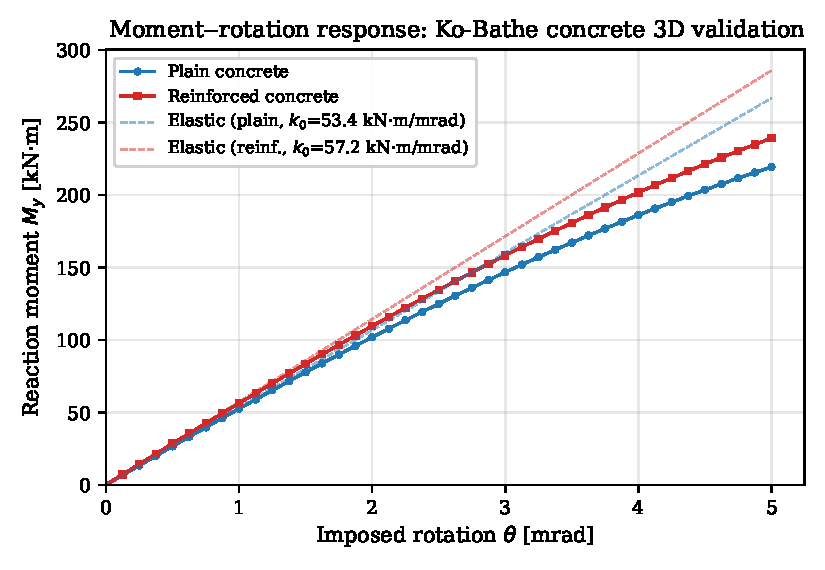
\includegraphics[width=0.95\textwidth]{figures/rc_beam_validation/moment_rotation.pdf}
  \caption{Moment--rotation response for plain and reinforced concrete beams.
           Dashed lines show the initial elastic stiffness.  Progressive
           cracking causes both curves to deviate from the elastic
           reference, with the reinforced beam maintaining consistently
           higher capacity.}
  \label{fig:rcbeam-moment-rotation}
\end{figure}

Key observations:
%
\begin{itemize}
  \item Both curves depart from the linear regime early as tensile
        cracking initiates in the extreme fibre, producing a gradual
        softening of the moment--rotation slope.
  \item The plain concrete beam reaches $M_y = 219.3$~kN$\cdot$m at
        $\theta = 5$~mrad; the reinforced beam reaches
        $M_y = 239.2$~kN$\cdot$m---a \textbf{9.1\% increase} from the
        embedded rebar.
  \item The initial elastic stiffness $k_0 = M_y / \theta$ is
        $53.4$~kN$\cdot$m/mrad (plain) and
        $57.2$~kN$\cdot$m/mrad (reinforced), consistent with beam
        theory for a doubly-clamped beam
        ($k = 4EI_y/L$, $I_y = h\,b^3\!/12$).
\end{itemize}


\subsection{Stiffness Degradation}
\label{sec:rcbeam-stiffness}

Figure~\ref{fig:rcbeam-stiffness} plots the tangent stiffness
$\mathrm{d}M/\mathrm{d}\theta$ at each step.  Both curves exhibit
monotonically decreasing stiffness as cracking progresses:

\begin{figure}[htbp]
  \centering
  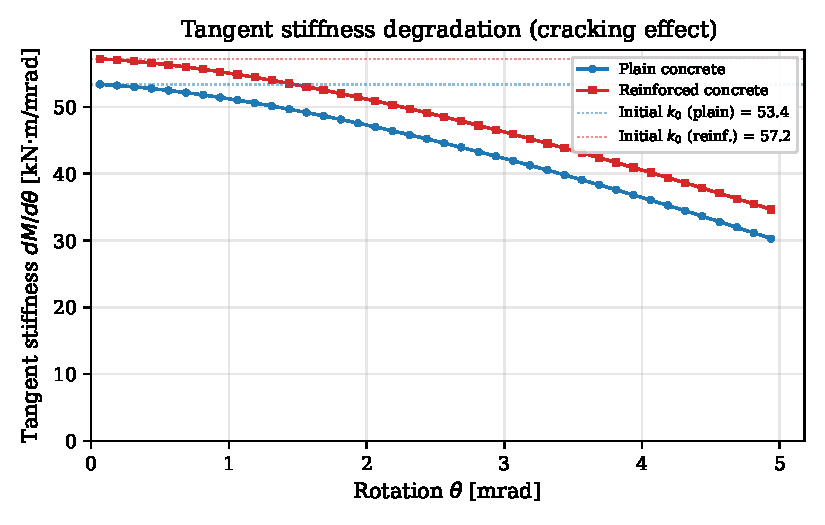
\includegraphics[width=0.95\textwidth]{figures/rc_beam_validation/stiffness_degradation.pdf}
  \caption{Tangent stiffness degradation showing the effect of
           progressive concrete cracking.  Dotted lines indicate the
           initial elastic stiffness.  The reinforced beam retains a
           higher tangent stiffness throughout the loading history.}
  \label{fig:rcbeam-stiffness}
\end{figure}

\begin{itemize}
  \item The plain concrete beam loses approximately 43\% of its initial
        stiffness by $\theta = 5$~mrad
        ($k_t$: $53.4 \to 30.3$~kN$\cdot$m/mrad).
  \item The reinforced beam loses approximately 39\% ($57.2 \to 34.7$),
        confirming the tension-stiffening effect of the embedded rebar:
        the steel carries tensile forces across cracks, partially
        restraining the stiffness degradation.
  \item The degradation profile is smooth and monotonic, with no abrupt
        jumps or oscillations, indicating that the Ko--Bathe smeared-crack
        model transitions between intact and cracked states in a
        numerically stable fashion.
\end{itemize}


\subsection{Moment Ratio}
\label{sec:rcbeam-ratio}

Figure~\ref{fig:rcbeam-ratio} shows the ratio
$M_y^{\text{reinf.}} / M_y^{\text{plain}}$ across the loading history.
The rebar contribution grows monotonically from 7.2\% to 9.1\% as
cracking progresses, because the steel carries an increasing share
of the tensile resultant as the concrete loses stiffness.

\begin{figure}[htbp]
  \centering
  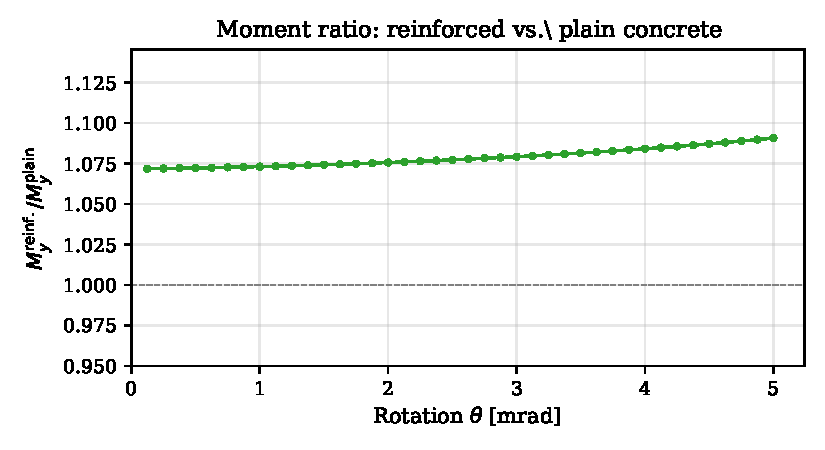
\includegraphics[width=0.85\textwidth]{figures/rc_beam_validation/moment_ratio.pdf}
  \caption{Ratio of the reinforced-to-plain moment capacity.
           The rebar contribution increases as cracking progresses.}
  \label{fig:rcbeam-ratio}
\end{figure}


% =========================================================================
\section{Analytical Cross-Check}
\label{sec:rcbeam-analytical}

For a doubly-clamped beam with an imposed rotation $\theta$ at one end,
Euler--Bernoulli beam theory gives the reaction moment at the rotating
end as
%
\begin{equation}\label{eq:rcbeam-elastic}
  M_y = \frac{4\,E\,I_y}{L}\,\theta,
  \qquad
  I_y = \frac{h\,b^3}{12} = \frac{0.40 \times 0.30^3}{12}
      = 9.0 \times 10^{-4}~\text{m}^4.
\end{equation}
%
Using the initial tangent stiffness $k_0 = 53.4$~kN$\cdot$m/mrad from
the simulation, the back-calculated Young's modulus is
%
\[
  E_0 = \frac{k_0 \, L}{4 \, I_y}
      = \frac{53{,}400 \times 2.0}{4 \times 9.0 \times 10^{-4}}
      \approx 29{,}667~\text{MPa},
\]
%
which is consistent with the Ko--Bathe model's initial elastic modulus
for $f'_c = 30$~MPa
(the ACI~318 formula gives $E_c = 4{,}700\sqrt{f'_c} \approx 25{,}743$~MPa;
the Eurocode~2 formula gives $E_{cm} = 22{,}000\,(f_{cm}/10)^{0.3}
\approx 32{,}837$~MPa for $f_{cm}=38$~MPa).  The back-calculated value
falls between these standard estimates, confirming that the Ko--Bathe
model uses a reasonable initial elastic modulus.

The smooth departure from the elastic reference in
Figure~\ref{fig:rcbeam-moment-rotation} is the expected signature of the
smeared-crack approach: the model does not exhibit a sharp cracking event
but rather a gradual redistribution of stresses as Gauss points
transition from intact to cracked states.


% =========================================================================
\section{Implementation Notes}
\label{sec:rcbeam-implementation}

The validation driver (\texttt{main\_rc\_beam\_validation.cpp}) is a
standalone executable that exercises the same infrastructure used by the
sub-model solver:

\begin{enumerate}
  \item \textbf{Mesh generation.}
        \texttt{make\_prismatic\_domain()} for Case~A;
        \texttt{make\_reinforced\_prismatic\_domain()} for Case~B.
        Both produce a \texttt{Domain<3>} + \texttt{PrismaticGrid} pair.

  \item \textbf{Element assembly.}
        Case~A uses a standard \texttt{Model} with homogeneous hex8
        elements.  Case~B builds a \texttt{std::vector<FEM\_Element>}
        with 256~hex8 and 128~truss elements, assembled via
        \texttt{MultiElementPolicy}.

  \item \textbf{Boundary conditions.}
        The rotation BCs are computed from the rigid-section kinematics
        formula~\eqref{eq:rcbeam-bc} and applied as Dirichlet constraints.
        The \texttt{CustomControl} scales the full displacement pattern
        by the load parameter~$p$.

  \item \textbf{Post-processing.}
        A step callback extracts the internal force vector at each
        converged increment, computes the resultant moment via
        Eq.~\eqref{eq:rcbeam-moment}, and records the data to CSV
        files.

  \item \textbf{VTK export.}
        Final-step meshes and Gauss-point fields are exported via
        \texttt{VTKModelExporter} for visualization.
\end{enumerate}

The entire pipeline runs in approximately 50~seconds per case on a
single core (no MPI parallelism required for this validation test).


% =========================================================================
\section{Conclusions}
\label{sec:rcbeam-conclusions}

The validation confirms that:

\begin{enumerate}
  \item The Ko--Bathe 3D constitutive model produces physically meaningful
        nonlinear responses under monotonic bending: gradual stiffness
        degradation from smeared cracking, consistent initial elastic
        modulus, and no spurious oscillations or loss of convergence.

  \item The \texttt{MultiElementPolicy} infrastructure correctly assembles
        heterogeneous hex8~+~truss element vectors, and the embedded
        rebar provides the expected tension-stiffening effect (7--9\%
        additional capacity at $\theta = 5$~mrad).

  \item The \texttt{CustomControl} displacement-control mechanism, which
        is the same mechanism used by \texttt{SubModelSolver}, reliably
        drives the incremental analysis through the full loading range
        without bisection.

  \item The back-calculated initial stiffness is consistent with
        standardised Young's modulus estimates for 30~MPa concrete,
        validating the Ko--Bathe model's elastic regime.
\end{enumerate}

These results provide confidence that the sub-model solver will produce
correct results when called from the multiscale analysis pipeline under
incrementally changing beam kinematics.
